% Motivacio, Leiras

 
 \section{Motiváció} 
 
	Korábban elvégzett atomerő mikroszkópos mérések (AFM) validálása során az
	alábbi probléma keletkezett.
	A fémezett felület topológiáját mérések eredményeként ismerjük adott
	pontossággal.
	A mérések egy négyzetes háló felett történtek, amelynek mindkét irányban ($xy$)
	azonos felbontása volt.
	A mérés során a fémezett felülettől mindig azonos távolságra lévő, hosszú hegyes tűre ható erőt mértük,
	amikor a felület és a tű között adott, állandó feszültséget kapcsoltunk.
	
	A tűre ható erőt mérve a felület tű alatti tartományban található töltéseloszlásról kapunk információt.
	Végső cél olyan szimulátor építése, amelynek segítségével közel valós időben 
	lehetséges felületmérés alapján a felületli töltéseloszlásról információt
	kapni.
	
	A cikkben felhasznált mérési eredmény (\ref{fig:felulet}. ábra) egy
	$512\times512$ méretű tömb, amely értékei $0-255$-ig terjed.
	
	\begin{figure}[!h]
		\centering
		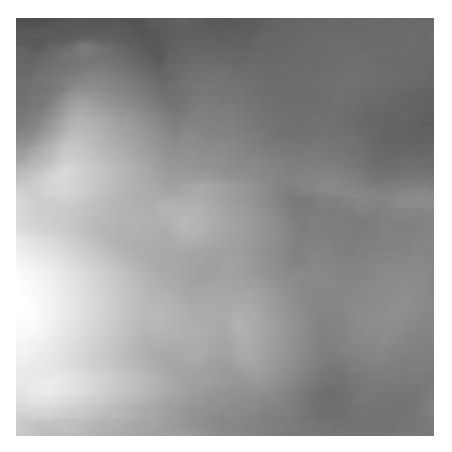
\includegraphics[width=0.45\columnwidth]{kepek/afm200.eps}
		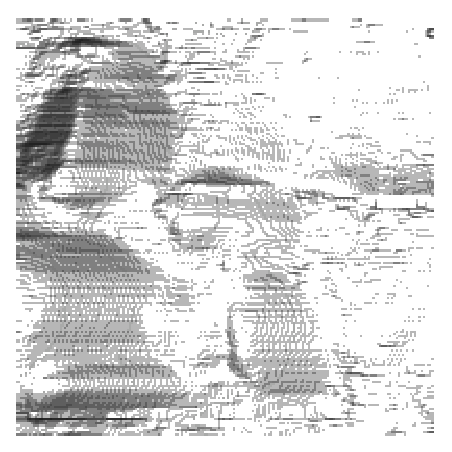
\includegraphics[width=0.45\columnwidth]{kepek/efm200.eps}
		\caption{Méréssel kapott felület (balra) és szimulációval kapott töltéstérkép}
		\label{fig:felulet}
	\end{figure}
	
	
	
	\section{Szimuláció} 
	
	\subsection{Fizikai probléma leírása} 
	
	A megoldandó feladat egy elektrosztatikus feladat.
	A  határfeltételek a felület fémezése, amely zérus potenciálú és az adott
	potenciálú ($U_{pot}$) tű fémes felülete.
	A határok többi részén homogén Neumann feltételt alkalmazhatunk a szimmetriák és a töltésmentesség miatt.
	
	A belső térben nincsenek töltések, így itt a Laplace-egyenlet érvényes
	\eqref{eq:1}.
	
	\begin{equation}\label{eq:1}
		\Delta \ U(x,y,z) = 0 
	\end{equation}
	
	Ennek megoldására lehetséges direkt és iteratív megoldó algoritmusokat alkalmazni.
	Mindkét módszer esetében a 3 dimenziós probléma esetében téren diszkretizáljuk a problémát,
	amelynek vízszintes felbontása $\Delta_x$ és $\Delta_y$, míg függőlegesen $\Delta_z$.
	Az így kapott térbeli háló minden pontjához hozzárendeljük az $U_{i,j,k}$ potenciált
	 ($1\leq i\leq i_{max}$, $1\leq j\leq j_{max}$, $1\leq k\leq k_{max}$). 
	
% 	Az alkalmazott interpoláció során a függőleges irányú felbontást is figyelembe véve 
	A párhuzamosítási szándékok miatt az iteratív megoldást választottuk.
	Ekkor nem teljesen pontos megoldást kapunk, azonban kevesebb lépéssel
	juthatunk el a kívánt eredményhez.
	A számítási pontosság növelhető keményebb konvergenci követelmény
	megszabásával, ami további iterációkat jelent.
	
	Az iteratív megoldás során a megoldás aktuális értékének kiszámításához az
	előző megoldásból indulunk ki.
	A \eqref{eq:2} alapján végezzük az iterációt.
		\begin{multline} \label{eq:2} 
			U_{ijk}^{n+1} = \\ \Delta_1 \cdot \left(U_{i-1,j,k}^n+U_{i+1,j,k}^n
			+U_{i,j-1,k}^n+U_{i,j+1,k}^n\right)+ \\
							\Delta_2 \cdot \left(U_{i,j,k-1}^n+U_{i,j,k+1}^n\right)
		\end{multline}
	ahol $U_{i,j,k}^n$ az az $n$-dik iterációs lépésben az $i,j,k$ koordinátájú
	pontban mérhető potenciált jelöli, $\Delta_1$ a vízszintes felbontásból,
	$\Delta_2$ a függőleges felbontásból adódó állandó.
	Az iterációs eljárás előnye, hogy implementációja egyszerűbb és a
	\eqref{eq:2} szerinti ``simítás'' gyorsabb, mint a direkt megoldás.
	%Az iterációs eljárás előnye, hogy memóriaigénye kicsi a direkt megoldás során
	% adódó egyenletmegoldáshoz képest.
	%Hátránya hogy nem ad pontos választ egy lépésben.
	
	\begin{figure}[!ht]
		\centering
		\psfrag{ijk}{$(i,j,k)$}
		\psfrag{imjk}{$(i-1,j,k)$} 
		\psfrag{ipjk}{$(i+1,j,k)$}
		\psfrag{ijmk}{$(i,j-1,k)$} 
		\psfrag{ijpk}{$(i,j+1,k)$}
		\psfrag{d1}{$k_x$} 
		\psfrag{d2}{$k_y$} 
		\psfrag{d3}{$k_z$} 
		\psfrag{ijkm}{$(i,j,k-1)$} 
		\psfrag{ijkp}{$(i,j,k+1)$} 
		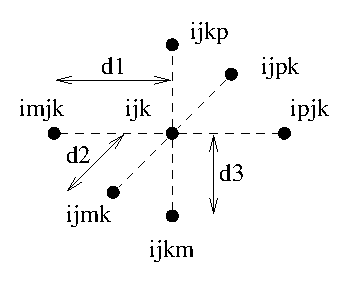
\includegraphics[width=0.95\columnwidth]{kepek/sema.eps}
		\caption{Diszkretizálás során alkalmazott felosztás} 
	\end{figure}

	
% 	fi(idx,idy,idz) = KK1*(fip(idx-1,idy,idz)+fip(idx+1,idy,idz)+fip(idx,idy-1,idz)+fip(idx,idy+1,idz))+...
%               KK2*(fip(idx,idy,idz-1)+fip(idx,idy,idz+1))

	\subsection{Szimuláció felépítése} 
	
	Mivel a Coulomb-kölcsönhatás a távolság négyzetével fordítottan arányos,
	így egy pont szomszédjait, pontosabban egy redukált környezetét szükséges
	csupán szimulálni.
	Ezzel az elhanyagolással már numerikusan kezelhető bonyulultságú problémára
	jutunk.
	
	Ezen módon egy mért pont $3\times3$-as környezetét vesszük figyelembe,
	a középső pont felett lévő felső elektródát feltételezve.
	A szimulációs felületen belül a mért magassági értékeket
	mint mintákat 2D-ben interpoláljuk.

	A szimulációk során a felület magasságának mérési adatait már ismertnek feltételezzük.
	A teljes mérőfelület pontjait külön-külön vizsgáljuk.
	Egyetlen pontban a mérési eredmény kiszámításának lépései az alábbiak :
	
	\begin{enumerate}
		\item A pont körüli felület $3\times3$-as mérési részének megállapítása,
		\item Közbenső (virtuális) mérési pontokkal a belső felbontás növelése
		interpolációval,
		\item Szimulálandó tér méretének számítása,
		\item Direkt/iteratív megoldó algoritmussal a tér meghatározása, 
				a tűre ható erő számítása illetve a tű alatti töltésmennyiség számítása,
		\item Adatok mentése.
	\end{enumerate}
	


	
